\documentclass{article}
\usepackage[utf8]{inputenc}
\usepackage{amsmath}
\usepackage{amsfonts}
\usepackage{geometry}
\usepackage{stmaryrd}
\usepackage[table]{xcolor}
\usepackage{fancybox}
\usepackage{tikz}
\usepackage{listings}
\usepackage{adjustbox}
\usepackage{amsmath}
\usetikzlibrary{positioning}
\geometry{a4paper,left=25mm,right=25mm,top=20mm}

\title{Planification du pompage dans un réseau de distribution d'eau potable ramifié\\-\\Optimisation non-linéaire en nombre entier}
\author{Robinson Beaucour}
\date{Décembre 2022}

\begin{document}

\maketitle

\begin{figure}[h]
    \centering
    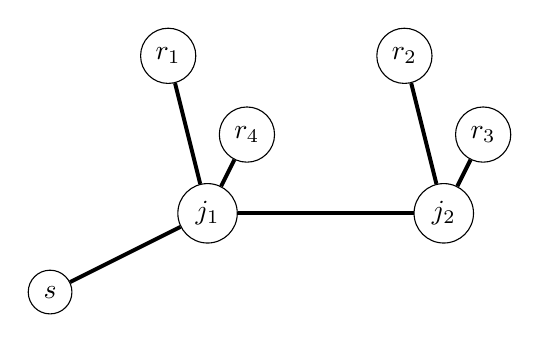
\begin{tikzpicture}[main/.style = {draw, circle}] 
        \node[main] (s) at (0,0) {$s$};
        \node[main] (j_1)   at (2,1)    {$j_1$}; 
        \node[main] (j_2)   at (5,1)    {$j_2$};
        \node[main] (r_1)   at (1.5,3)  {$r_1$};
        \node[main] (r_4)   at (2.5,2)  {$r_4$};
        \node[main] (r_2)   at (4.5,3)  {$r_2$};
        \node[main] (r_3)   at (5.5,2)  {$r_3$};
        \draw   [line width=0.5mm]  (s)     --  (j_1);
        \draw   [line width=0.5mm]  (j_1)   --  (j_2);
        \draw   [line width=0.5mm]  (j_1)   --  (r_1);
        \draw   [line width=0.5mm]  (j_1)   --  (r_4);
        \draw   [line width=0.5mm]  (j_2)   --  (r_2);
        \draw   [line width=0.5mm]  (j_2)   --  (r_3);
    \end{tikzpicture}
    \caption{Réseau de distribution simple}
\end{figure}

\paragraph{Variables de décision}
$$
\left.
    \begin{array}{lll}
        Q_{pompe,t}^{(k)}       &   \text{Débit sortant de la pompe $k$ à l'instant $t$}    & [Q_{min}^{(k)},Q_{max}^{(k)}]\cup\{0\}\\[0.2cm]
        Q_{reserv,t}^{(r)}      &   \text{Débit entrant du réservoire $r$ à l'instant $t$}  & \mathbb{R}_+\\[0.2cm]
        Q_{jonction,t}^{(n,n')}   &   \text{Débit dans le tuyau allant du noeud $n$ au $n'$ à l'instant $t$}  &   \mathbb{R}_+\\[0.2cm]
        C_t^{(n)}               &   \text{Niveau de charge (en m) au noeud $n$}             & \mathbb{R}_+\\[0.2cm]
        G_{pompe,t}^{(k)}       &   \text{Gain de charge de la pompe $k$ à l'instant $t$}   & \mathbb{R}_+\\[0.2cm]
        P_{pompe,t}^{(k)}       &   \text{Puissance électrique consommée par la pompe $k$ à l'instant $t$}& \mathbb{R}_+\\[0.2cm]
        V_t^{(r)}               &   \text{Volume du réservoire $r$ à l'instant $t$}& [V_{min}^{(r)},V_{max}^{(r)}]\\[0.2cm]
        S_{on,t}^{(k)}          &   \text{Etat de la pompe $k$ (allumé/éteint) à l'instant $t$}&\{0,1\}\\[0.2cm]
    \end{array}
\right.
$$
\paragraph{Contraintes}
\begin{equation}
    \tag{Equilibre flux}  
    \left.
        \begin{array}{lcccc}
            \forall t,\forall j   &   \sum_{n} Q_{jonction,t}^{(n,j)}    & = &   \sum_{n} Q_{jonction,t}^{(j,n)}\\[0.2cm]
        \end{array}
    \right.
\end{equation}

\begin{equation}
    \tag{Satisfaction demande}  
    \left.
        \begin{array}{lcccc}
            \forall t, \forall r   &   V_{t+1}^{(r)}-V_t^{(r)}     & = &   Q_{reserv,t}^{(r)} - D_t^{(r)}\\[0.2cm]
        \end{array}
    \right.
\end{equation}
    
\begin{equation}
    \tag{Conso. élec pompe}  
    \left.
        \begin{array}{lccc}
            \forall t, \forall k   &   P_{pompe,t}^{(k)}     & \geq &   \Gamma_0^{k}S_{on,t}^{(k)} + \Gamma_1^{(k)}Q_{pompe,t}^{(k)}\\[0.2cm]
        \end{array}
    \right.
\end{equation}

\begin{equation}
    \tag{Gain charge pompe}
    \left.
        \begin{array}{lccc}
            \forall t, \forall k   &   G_{pompe,t}^{(k)}     & \leq &   \psi_0^{k}S_{on,t}^{(k)} + \psi_2^{(k)}(Q_{pompe,t}^{(k)})^2\\[0.2cm]
        \end{array}
    \right.
\end{equation}

\begin{equation}
    \tag{Perte charge flux}
    \left.
        \begin{array}{lcccc}
            \forall t, \forall n,n'   &   C_t^{(n)}  - C_t^{(n')}    & = &   \phi_1^{(n,n')}Q_{jonction,t}^{(n,n')} + \phi_2^{(n,n')}(Q_{jonction,t}^{(n,n')})^2\\[0.2cm]
        \end{array}
    \right.
\end{equation}

\begin{equation}
    \tag{Charge source}
    \left.
        \begin{array}{lcccc}
            \forall t, \forall n,n'   &   0 & \leq & (\sum_k S_{on,t}^{(k)})    (G_{pompe,t}^{(k)}-C_t^{(s)})\\[0.2cm]
        \end{array}
    \right.
\end{equation}

\begin{equation}
    \tag{Charge jonction}
    \left.
        \begin{array}{lcccc}
            \forall t, \forall j   &   C_t^{(j)}    & \geq &   H^{(j)}\\[0.2cm]
        \end{array}
    \right.
\end{equation}

\begin{equation}
    \tag{Charge réservoire}
    \left.
        \begin{array}{lcccc}
            \forall t, \forall r   &   C_t^{(r)}    & \geq &   H^{(j)}\\[0.2cm]
        \end{array}
    \right.
\end{equation}
    
% \underline{GAMS :}\\
\begin{adjustbox}{max width=\textwidth}
    \begin{lstlisting}
        Noeud(j,t) .. sum(n$l(j,n), Qpipe(j,n,t)) =e=  sum(n$l(n,j), Qpipe(n,j,t));
        Satisfaction_demande(r,t) ..  v(r,t) - v(r,t-1) - vinit(r,t) =e= 1 * (sum=(n$l(n,r),Qpipe(n,r,t))-demand(r,t));
        Elec_pompe(k(c,d),t) .. Ppompe(k,t) =g=  gamma(c,"0") * Son(k,t) + gamma(c,"1")*Qpompe(k,t);
        Gain_charge_pompe(k(c,d),t) .. Gpompe(k,t) =l= psi(c,"0") * Son(k,t) + psi(c,"2")*Qpompe(k,t)**2;
        Charge_s("s",t) .. 0 =l= (sum(k, Gpompe(k,t))-Charge("s",t))*sum(k, Son(k,t));
    \end{lstlisting}
\end{adjustbox}

\paragraph{Objectif}
$$
    \text{Minimiser }   \sum_t \sum_k P_{pompe,t}^{(k)}\cdot C_t
$$
\end{document}
